\chapter{Discussão das técnicas em um contexto aplicado}

Neste Capítulo serão contextualizadas as técnicas emergentes de teste de software, assim como serão feitas discussões sobre os pontos em aberto acerca de tais técnicas. Será utilizado como base para estas contextualizações e discussões o código e experiências envolvidas no desenvolvimento do kanban-roots, agregando uma visão prática e aplicada à um projeto real.

\section{O kanban-roots}
\label{sec:kanban_roots}

O kanban-roots é um kanban\footnote{O termo tem origem no sistema Toyota de produção, onde kanban é a maneira como é coordenado o fluxo de peças na cadeia de suprimentos  \cite{AMaquinaQueMudouOMundo}. No contexto do presente trabalho, kanban é um quadro para visualização do fluxo de trabalho (tarefas) em um projeto.} online para auxiliar a organização e acompanhamento das tarefas em um projeto, sendo especialmente interessante para projetos \textit{opensouce} ou, de modo geral, para projetos com equipes geograficamente distribuídas.

Na figura \ref{img:tela_kaban_roots} pode ser visto um \textit{screen shot} do kanban de um projeto no kanban-roots.

O kanban é muito utilizado em metodologias ágeis como XP e Scrum como um quadro para visualização do fluxo de tarefas nas iterações de um projeto. As tarefas inicialmente são posicionadas na divisão \textbf{\textit{Backlog}} até serem escolhidas para fazer parte de uma iteração. Nesse momento, as tarefas escolhidas vão para a divisão \textbf{\textit{To Do}} até que sejam escolhidas por um desenvolvedor para serem implementadas, passando para a divisão \textbf{\textit{Doing}}. Após o desenvolvedor concluir a tarefa, esta vai para a divisão \textbf{\textit{Done}}. Dessa maneira, todos os participantes tem a possibilidade de ver como está o andamento da iteração, além de ser possível acompanhar o que cada integrante do projeto está está fazendo naquele instante.

O kanban-roots já está em produção e vem sendo testado e utilizado com sucesso por algumas pessoas em empresas do Brasil como a Algorich, Voxline, Mandic, Quatix, mas também estrangeiras como a infoPiiaf e Free.fr (França), Ginzametrics (Estados Unidos), Osube (China), Centah (Canadá), Podmoskovie.info (Rússia), EvoEnergy (Inglaterra), Forgotten Labs (Lituânia), entre outros.

\begin{figure}[h]
  \center
  \caption{Tela do kanban de um projeto no kanban-roots}
  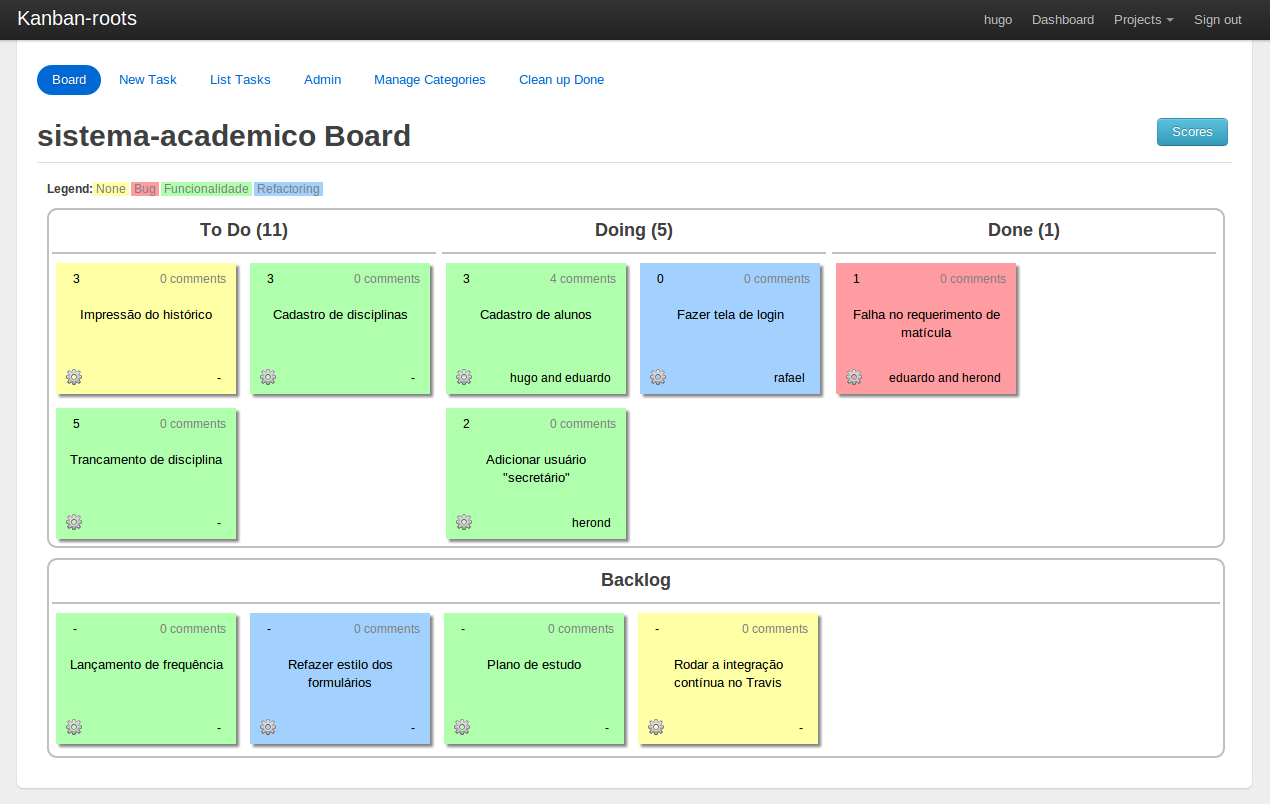
\includegraphics[scale=0.35]{images/kanban-roots}
  \label{img:tela_kaban_roots}
\end{figure}

\section{Contextualizando TDD}
\label{sec:contextualizando_tdd}

Para apresentar como a utilização do TDD se dá na prática, serão mostrados os passos para a implementação da seguinte funcionalidade chave para a montagem kanban:

\begin{quote}
\textit{Precisa-se saber todas as tarefas posicionadas em uma determinada posição do kanban (quadro) de um projeto.}
\end{quote}

A primeira coisa a ser feita é o teste para o caso mais simples: quando o projeto não tem tarefa alguma naquela determinada posição do kanban.

Desta forma, o teste de unidade para o caso mais simples pode ser como mostrado no Código \ref{code:tdd_test1}, onde é criada uma instância da classe \texttt{Project} e é feita uma asserção de que não tem tarefas na posição 4 do quadro.

\begin{mycode}{ruby}%
{Teste para o método Project\#tasks\_by\_position (versão 1)}{code:tdd_test1}
# test/unit/project_test.rb
class ProjectTest < ActiveSupport::TestCase
  def test_tasks_by_position
    project = Factory.create :project
    assert_equal(project.tasks_by_position("done"), [])
  end
end
\end{mycode}

Ao rodar este teste, ele irá falhar, informando que o método \texttt{tasks\_by\_position} sequer existe. Como esta era a falha esperada, é escrito então o código mais simples para passar neste teste, apresentado no Código \ref{code:tdd_code1}, onde apenas é retornada uma lista vazia.

\begin{mycode}{ruby}%
{Implementação do método Project\#tasks\_by\_position (versão 1)}{code:tdd_code1}
# app/models/project.rb
def tasks_by_position position
  []
end
\end{mycode}

Os testes irão passar. Mas a funcionalidade ainda não está completa e, consequentemente, o teste também não. Como pode ser visto no Código \ref{code:tdd_test2}, é adicionado ao teste uma verificação de que para a posição 1 devem existir duas tarefas e que estas tarefas devem ser exatamente as criadas anteriormente.

\begin{mycode}{ruby}%
{Teste do método Project\#tasks\_by\_position (versão 2)}{code:tdd_test2}
# test/unit/project_test.rb
class ProjectTest < ActiveSupport::TestCase
  def test_tasks_by_position
    project = Factory.create :project
    tasks = [Factory.create(:task, :project => project, :position => "backlog"),
             Factory.create(:task, :project => project, :position => "backlog")]

    assert_equal(project.tasks_by_position("done"), [])

    assert_equal(project.tasks_by_position("backlog").count, 2)
    tasks.each { |task| assert(project.tasks_by_position("backlog").include?(task)) }
  end
end
\end{mycode}

Como o teste foi alterado, este é executado e irá falhar, informando que na \hyperref[code:tdd_test2]{linha 10} eram esperadas duas tarefas, mas foram obtidas zero. O código então deve ser modificado para passar no novo teste e é apresentado no código \ref{code:tdd_code2}.

\begin{mycode}{ruby}%
{Implementação do método Project\#tasks\_by\_position (versão 2)}{code:tdd_code2}
# app/models/project.rb
def tasks_by_position position
  task_list = []
  tasks.each do |task|
    task_list << task if task.position == position
  end
  task_list
end
\end{mycode}

Desta vez, após a modificação no código e a execução dos testes, todos os testes os irão passar. Contudo, a cobertura de testes para este método ainda está fraca, o que pode ser resolvido com a adição de mais algumas tarefas em posições diferentes, como mostrado no Código \ref{code:tdd_test3}.

\begin{mycode}{ruby}%
{Teste do método Project\#tasks\_by\_position (versão 3)}{code:tdd_test3}
# test/unit/project_test.rb
class ProjectTest < ActiveSupport::TestCase
  def test_tasks_by_position
    project = Factory.create :project
    tasks = [Factory.create(:task, :project => project, :position => "backlog"),
             Factory.create(:task, :project => project, :position => "backlog"),
             Factory.create(:task, :project => project, :position => "todo"),
             Factory.create(:task, :project => project, :position => "doing"),
             Factory.create(:task, :project => project, :position => "doing")]

    assert_equal(project.tasks_by_position("done"), [])

    assert_equal(project.tasks_by_position("backlog").count, 2)
    tasks[0..1].each { |task| assert(project.tasks_by_position("backlog").include?(task)) }

    assert_equal(project.tasks_by_position("todo"), [tasks[2]])

    assert_equal(project.tasks_by_position("doing").count, 2)
    tasks[3..4].each { |task| assert(project.tasks_by_position("doing").include?(task)) }
  end
end
\end{mycode}

Executando os testes novamente, todos eles passam, como mostrado na figura \ref{img:test-unit-exec}. Isto indica que já é hora de ir para o item 5 do ciclo TDD e refatorar. Ao comparar o Código \ref{code:tdd_code2} com sua versão refatorada, apresentada no Código \ref{code:tdd_code3}, pode-se perceber como a segunda está mais simples e clara e que ao rodar os testes, estes passam mostrando que o comportamento do método não mudou.

\begin{mycode}{ruby}%
{Implementação do método Project\#tasks\_by\_position (versão 3)}{code:tdd_code3}
# app/models/project.rb
def tasks_by_position position
  tasks.select { |item| item.position == position }
end
\end{mycode}

\begin{figure}[h]
  \center
  \caption{Saída produzida pela execução dos testes de unidade com utilizando TDD com testUnit}
  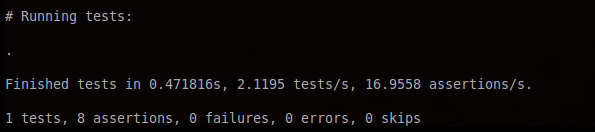
\includegraphics[scale=0.6]{images/test-unit-exec}
  \label{img:test-unit-exec}
\end{figure}

Com isso, o ciclo TDD para o desenvolvimento da funcionalidade é terminado, produzindo um código legível, limpo e bem coberto por testes, como pode ser visto no Código \ref{code:tdd_code3}. Além disso, o código faz exatamente o que se espera dele, nada a mais nem nada a menos, atendendo os requisitos definidos nos testes, que são apresentados no Código \ref{code:tdd_test3}.

Outro exemplo, neste caso de teste de integração, é o de uma extensão criada para fazer o destaque da sintaxe (\textit{highlighting}) de código na descrição das Tarefas e no conteúdo do Comentários no kanban-roots, como apresentado na Figura \ref{img:highlighting}. Para isso, é utilizado um \textit{framework} em Python chamado Pygments\footnote{ Mais em \url{http://pygments.org/}}, que recebe como parâmetros uma \textit{string} com o código a ser destacado e a linguagem em que este código está escrito, retornando uma nova \texttt{string} em html com o código destacado.

\begin{figure}[h]
  \center
  \caption{Comentário com destaque da sintaxe de código no kanban-roots}
  \includegraphics[scale=0.5]{images/highlighting}
  \label{img:highlighting}
\end{figure}

O Pygments deve ser instalado na máquina onde o kanban-roots está sendo executado. No entanto, o kanban-roots foi projetado rodar tanto em um servidor próprio ou em um VPS\footnote{ \textit{Virtual Private Server}. É um servidor em ambiente compartilhado que possui acesso \textit{root} e processos independentes para cada conta VPS criada.}, como também no Heroku\footnote{ É um PaaS (\textit{platafom as a service}) que tem uma cota de utilização gratuita. No Heroku não é possível instalar dependências no sistema. Mais em \url{http://heroku.com}}. Sendo assim, além da possibilidade de utilizar o Pygments instalado localmente, foi utilizado um serviço gratuito e não oficial criado por Trevor Turk e hospedado no Google App Engine (GAE)\nomenclature{GAE}{Google App Engine} que permite a utilização da API \nomenclature{API}{Application programming interface} do Pygments através de uma requisição (através do método HTTP POST) para o serviço. \textbf{Dessa forma, deve-se testar a integração do kanban-roots com o Pygments instalado localmente e também com o serviço externo hospedado no GAE}.

Primeiramente, é feito o teste para o caso em que o Pygments é instalado localmente, apresentado no Código \ref{code:integration_spec1}.

\begin{mycode}{rspec}%
{Teste de integração para o \textit{highlighting} de código (versão 1)}{code:integration_spec1}
# spec/lib/albino_render_spec.rb
describe HTMLwithAlbino do
  it "should get the highlighted block code from local pygments" do
    render = HTMLwithAlbino.new
    render.block_code('puts "hello!"', "ruby").should ==
      "<div class=\"highlight\"><pre>" +
        "<span class=\"nb\">puts</span> <span class=\"s2\">&quot;hello!&quot;</span>\n" +
      "</pre>\n</div>\n"
  end
end
\end{mycode}

A implementação para este teste é apresentado no Código \ref{code:integration1}, onde o método \texttt{colorize} da classe \texttt{Albino} invoca o Pygments do sistema.

\begin{mycode}{ruby}%
{Implementação do \textit{highlighting} de código (versão 1)}{code:integration1}
# lib/albino_render.rb
class HTMLwithAlbino < Redcarpet::Render::HTML
  def block_code(code, lang)
    Albino.colorize(code, lang)
  end
end
\end{mycode}

Ao executar o teste, este passa. Como não tem nada para refatorar, é adicionado um novo teste para o caso em que o Pygments não está instalado no servidor, como é apresentado no Código \ref{code:integration_spec2}.

É importante perceber que foi utilizado um dublê de teste (neste caso um \textit{stub}) para simular a resposta do método \texttt{can\_pygmentize?} que fará uma verificação no sistema operacional para identificar se o Pygments está instalado ou não.

\begin{mycode}{rspec}%
{Teste de integração para o \textit{highlighting} de código (versão 2)}{code:integration_spec2}
# spec/lib/albino_render_spec.rb
describe HTMLwithAlbino do
  it "should get the highlighted block code from local pygments" do
    @render.stub(:can_pygmentize?).and_return(true)
    render = HTMLwithAlbino.new
    render.block_code('puts "hello!"', "ruby").should ==
      "<div class=\"highlight\"><pre>" +
        "<span class=\"nb\">puts</span> <span class=\"s2\">&quot;hello!&quot;</span>\n" +
      "</pre>\n</div>\n"
  end

  it "should get the highlighted block code from pygments.appspot.com" do
    @render.stub(:can_pygmentize?).and_return(false)
    render = HTMLwithAlbino.new
    render.block_code('puts "hello!"', "ruby").should ==
      "<div class=\"highlight\"><pre>" +
        "<span class=\"nb\">puts</span> <span class=\"s2\">&quot;hello!&quot;</span>\n" +
      "</pre>\n</div>\n"
  end
end
\end{mycode}

O Código \ref{code:integration2} apresenta a implementação que faz os dois casos de teste passarem. Nessa nova versão, foi preciso criar o método de suporte \texttt{can\_pygmentize?} que, como dito anteriormente, verifica se o Pygments está instalado. Se o Pygments estiver instalado, ele é invocado da mesma forma como na versão 1 da implementação. Porém, se o Pygments não estiver instalado, é feita uma requisição ao serviço externo.

\begin{mycode}{ruby}%
{Implementação do \textit{highlighting} de código (versão 2)}{code:integration2}
# lib/albino_render.rb
class HTMLwithAlbino < Redcarpet::Render::HTML
  def block_code(code, lang)
    if can_pygmentize?
      Albino.colorize(code, lang)
    else
      # This is a hack for pygments work on Heroku
      require "net/http"
      Net::HTTP.post_form(URI.parse("http://pygments.appspot.com/"),
                          {"code"=>code, "lang"=>lang}).body
    end
  end

  private
  def can_pygmentize?
    system "pygmentize -V"
  end
end
\end{mycode}

Como ao executar os testes, todos eles passam, podemos refatorar o código. Na implementação não há nada a ser refatorado, contudo, existe diversas duplicidades nos testes. O Código \ref{code:integration_spec3} apresenta os testes refatorados, eliminando as duplicidades com a ajuda do método \texttt{before} que, ao receber o \texttt{:all} como parâmetro, é executado antes de de todos os casos de teste.

\begin{mycode}{rspec}%
{Teste de integração para o \textit{highlighting} de código (versão 3)}{code:integration_spec3}
# spec/lib/albino_render_spec.rb
describe HTMLwithAlbino do
  before(:all) do
    @render = HTMLwithAlbino.new
    @code_text = 'puts "hello!"'
    @highlighted_code =
      "<div class=\"highlight\"><pre>" +
        "<span class=\"nb\">puts</span> <span class=\"s2\">&quot;hello!&quot;</span>\n" +
      "</pre>\n</div>\n"
  end

  it "should get the highlighted block code from local pygments" do
    @render.stub(:can_pygmentize?).and_return(true)
    @render.block_code(@code_text, "ruby").should == @highlighted_code
  end

  it "should get the highlighted block code from pygments.appspot.com" do
    @render.stub(:can_pygmentize?).and_return(false)
    @render.block_code(@code_text, "ruby").should == @highlighted_code
  end
end
\end{mycode}

Desta forma, mostra-se que não apenas o código da implementação deve ser refatorado, mas também o código dos testes. Assim como o código da implementação, o código dos testes devem ser igualmente legíveis e otimizados, pois também sofrem manutenção e precisam ser executados com rapidez.

É importante lembrar que foram omitidos alguns casos de teste para esta funcionalidade, como por exemplo, o caso em que existe uma falha na requisição ao serviço externo. Esta omissão foi feita para que não o exemplo não ficasse muito extenso, e por este já cumprir seu objetivo.


\subsection{Design emergente no kanban-roots}
\label{sub:design_emergente_no_kanban_roots}

Para o desenvolvimento do kanban-roots, foi de extrema importância que o design evoluísse incrementalmente, pois não se sabia ao certo que
funcionalidades seriam contempladas nem que entidades existiriam.

As entidades \textit{Project} e \textit{Contributor} tinham uma relação direta, n para n, como apresentado na Figura \ref{img:contributor_projetc}. Contudo, em um determinado momento achou-se pertinente a criação de uma nova entidade \textit{Team} que faria a ligação entre as outras duas entidades, como apresentado na Figura \ref{img:contributor_team_projetc}. Isto acarretou uma série de alterações \cite{CommitAddTeam}, dentre outras, na interface das entidades e na estrutura do banco de dados $-$ considerada uma alteração crítica, mas que com ferramentas como \textit{migrations},\footnote{\textit{Migrations} são uma forma conveniente de gerenciar bases de dados de maneira estruturada e organizada. Mais em \url{http://guides.rubyonrails.org/migrations.html}} torna-se simples.

\begin{figure}[h]
  \center
  \caption{Diagrama de classes relacionando \textit{Contributor} e \textit{Project}}
  \includegraphics[scale=0.28]{images/contributor_projetc}
  \label{img:contributor_projetc}
\end{figure}

Meses depois, foi verificado que esta entidade \textit{Team} não era mais necessária, acarretando novamente em diversas modificações \cite{CommitRemoveTeam}, voltando ao estado apresentado na Figura \ref{img:contributor_projetc}.

\begin{figure}[h]
  \center
  \caption{Diagrama de classes relacionando \textit{Contributor}, \textit{Team} e \textit{Project}}
  \includegraphics[scale=0.25]{images/contributor_team_projetc}
  \label{img:contributor_team_projetc}
\end{figure}

Foram diversas as situações em que mudanças como essa ocorreram durante o desenvolvimento do kanban-roots. Sem o suporte do TDD seria extremamente complicado fazer essas alterações e deixar o design emergir, pois a insegurança de que as modificações pudesse afetar outras partes do código seria muito grande. Além disso, a criação a priori dos testes favoreceu que as modificações fossem feitas de maneira mais simples, direta e rápida.

\subsection{A ubiquidade do TDD}
\label{sub:a_ubiquidade_do_tdd}

Existe uma controvérsia sobre a não utilização do TDD em qualquer situação. É dito ``sobre a \textbf{não} utilização"\ pois o autor desconhece qualquer literatura dizendo que TDD deve ser utilizado sempre e em qualquer situação. Porém, muitos defendem a sua não utilização em algumas situações como em fase de descobertas, em fase de experimentos, se o desenvolvedor nunca utilizou a API, se o código não será utilizado novamente ou se levar mais tempo para escrever os testes do que para escrever e executar o código.

\citeonline{CleanCode} define As Três Leis do TDD, onde a primeira delas é: ``Você não pode escrever código de produção até que você tenha escrito um teste de unidade com falha.". Deve-se ter bastante atenção para o trecho ``de produção", pois sem ele, o sentido da frase é completamente distorcido, dando a impressão de que deve-se utilizar em todas as situações.

Introduzindo o kanban-roots na discussão, nos dois únicos casos em que ocorreu um \textit{bug} em produção, ao ser feita uma analise no código em busca da solução, foi encontrado um comentário ``TODO: Make test and refactor"\ nos métodos onde os \textit{bugs} ocorreram. Atualmente, existem 5 comentários semelhantes a esse espalhados no código do kanban-roots. Isso, de certa forma, comprova que caso os testes não sejam escritos antes, para um código que irá entrar em produção, escrevê-lo depois acaba sendo um fardo, e isso é ignorado até que um problema ocorra.

Um exemplo para esta situação é apresentado no Código \ref{code:todo}, onde é mostrado um método de \textit{controller}\footnote{O \textit{controller} é um componente do padrão MVC (do inglês \textit{Model View Controller}) de desenvolvimento de software. Neste padrão, a lógica da aplicação (\textit{Model}) é isolada da interface do usuário (\textit{View}) através de um controlador (\textit{Controller}).} que é chamado via Ajax e implementa a atualização dos pontos de uma tarefa diretamente do kanban do projeto. Além de atualizar os pontos da tarefa na base de dados, este método captura, trata e envia informações para que a interface do kanban seja atualizada. Este foi um típico caso onde um experimento foi para produção, sem testes e com um código \textbf{extremamente ruim}.

\begin{mycode}{ruby}%
{Código do método que atualiza os pontos de uma tarefa diretamente do kanban do projeto}{code:todo}
# app/controllers/boards_controller.rb
class BoardsController < InheritedResources::Base
  # TODO: Make test and refactor
  def update_points
    task = Task.find(params[:task_id])
    points = params[:points] == '-' ? nil : params[:points]

    position = Board::POSITIONS.key(task.position)
    if position != 'done'
      score = 0
    else
      if task.points.nil?
        old_points = 0
      elsif task.points.zero?
        old_points = 0.1
      else
        old_points = task.points
      end
      if points.nil?
        new_points = 0
      elsif points.to_i.zero?
        new_points = 0.1
      else
        new_points = points.to_i
      end
      score = new_points - old_points
    end

    task.update_attribute(:points, points)

    project = Project.find(task.project_id)
    division_name = Board::POSITIONS[params[:division_id]]
    division_points = project.count_points(division_name)
    contributors = task.contributor_ids
    data = { :division_points => division_points,
             :contributors => contributors,
             :score => score }
    render :text => data.to_json
  end
end
\end{mycode}

Códigos como o apresentado acima são extremamente difíceis de serem testados, pois, além de possuir complexidade ciclomática acima do aceitável, desempenham tarefas de responsabilidade de outras unidades do software, o que aumenta em muito o seu acoplamento e dificulta a escrita dos testes. Se este código fosse escrito utilizando TDD, certamente estaria melhor escrito e com mais qualidade, pois para escrever o teste, o código teria que ser refatorado de modo a distribuir as diferentes responsabilidades incorporadas no mesmo. Assim, fica clara a íntima relação entre teste e implementação no que tange ao design e à qualidade.

\citeonline{LegacyCode} define que \textbf{código legado é código sem testes}. Esta afirmação, que pode parecer extremada, é simplesmente a constatação de que, sem uma ampla cobertura de testes automatizados, e uma vez que é economicamente inviável a aplicação manual de todos os casos de teste $-$ ou mesmo de parte deles $-$ de um software a cada modificação, é muito difícil ter uma margem razoável de segurança de que uma modificação não irá introduzir \textit{bugs} no software. Deste modo, para um código ``que irá para produção"\ a utilização do TDD é essencial, pois do contrário, se está criando código legado. É importante lembrar que o código legado com o tempo vai minando a manutenibilidade do sistema e assim, elevando os custos de introdução de novas funcionalidade e evolução do mesmo.

Conclui-se que, para quem adota TDD, somente nos casos em que um código será posteriormente eliminado, como em provas de conceito temporárias ou experimentos, a utilização da técnica não é invariavelmente necessária. Contudo, a utilização de TDD nesses cenários pode ser muito interessante, pois como dito anteriormente, para a escrita dos testes, é preciso entender bem o problema a ser resolvido, fazendo o desenvolvedor se preparar mais para o que ele ainda não conhece muito bem.


\section{Contextualizando BDD}

Nesta seção será visto como se dá a utilização do BDD se dá na prática, bem como sua relação com TDD, além de uma discussão acerca dos modelos de escrita dos testes com a utilização desta técnica.

\subsection{A relação entre BDD e TDD}
\label{sub:a_relacao_entre_bdd_e_tdd}

Como dito a anteriormente, BDD é uma evolução do TDD. A grande diferença entre os dois é que TDD não abrange a validação do software, ou seja, se o software atende os requisitos. Isso muda tudo, pois em BDD, a ênfase está no comportamento, e não na estrutura. Ao invés de focar em classes e métodos ao escrever os testes, o foco é no comportamento que gera valor para o sistema. Além disso, o pensamento não é voltado à verificação, mas sim no comportamento, em validar que o software faz sem deixar também de verificar se está funcionando como deveria.

Em BDD não são escritos testes, mas sim especificações, chamadas de \textit{specs} (de \textit{specifications}). Pode-se ter a clara diferença entre testes (TDD) e specs (BDD) comparando o Código \ref{code:tdd_test3} com o Código \ref{code:bdd_spec}, onde palavras chave como \textit{class}, \textit{test} e \textit{assert} dão lugar a \textit{describe}, \textit{it} e \textit{should}, ficando nítido o foco no comportamento. Além disso, a substituição do Test::Unit (TDD) pelo Rspec (BDD) também revela grande mudança nas asserções onde os \textit{asserts} dão lugar aos \textit{matchers}, fazendo com que as asserções possam ser lidas quase como uma linguagem natural.

\begin{mycode}{rspec}%
{Exemplo de uma spec}{code:bdd_spec}
# spec/models/project.rb
describe Project do
  it "returns all related tasks matching a given position" do
    project = Factory.create :project
    tasks = [Factory.create(:task, :project => project, :position => 1),
             Factory.create(:task, :project => project, :position => 1),
             Factory.create(:task, :project => project, :position => 2),
             Factory.create(:task, :project => project, :position => 3),
             Factory.create(:task, :project => project, :position => 3)]

    project.tasks_by_position(4).should be_empty

    project.should have(2).tasks_by_position(1)
    project.tasks_by_position(1).should include(*tasks[0..1])

    project.tasks_by_position(2).should == [tasks[2]]

    project.should have(2).tasks_by_position(3)
    project.tasks_by_position(3).should include(*tasks[3..4])
  end
end
\end{mycode}

Em TDD, o nome dos testes é baseado na estrutura do código, e isso pode ter um efeito colateral: criar duplicações. Ao escrever testes como o \texttt{test\_tesks\_by\_position} do Código \ref{code:tdd_test3} e o método \texttt{tasks\_by\_position} é renomeado, o nome do teste também terá que ser renomeado, o que na maioria das vezes é esquecido. Isso torna os testes confusos e desinformativos \cite{ContinuousTesting}. Como por definição, refatorar é melhorar a estrutura e o design do código sem alterar seu comportamento, nomeando os testes com base no comportamento desejado ao invés da estrutura do código, não apenas torna os testes mais informativos como também torna a refatoração menos custosa \cite{ContinuousTesting}.

% subsection a_relacao_entre_bdd_e_tdd (end)


\subsection{Modelos de escrita dos testes de aceitação}
\label{sub:modelos_de_escrita_dos_testes_de_aceitacao}

Existem duas maneiras principais de se escrever os testes de aceitação: em texto plano e em código puro. Para exemplificar cada uma das abordagens, será especificada a seguinte funcionalidade:

\begin{quote}
\textit{Os comentários mostrados na página de tarefas devem ser renderizados utilizando a linguagem de marcação Markdown.}
\end{quote}

O resultado desta funcionalidade implementada é apresentado na Figura \ref{img:markdown}.

\begin{figure}[h]
  \center
  \caption{Comentários renderizados com Markdown no kanban-roots}
  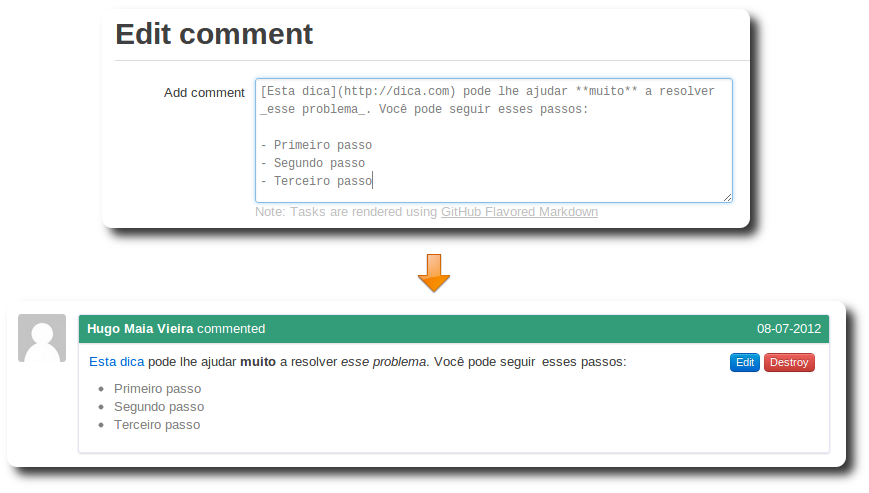
\includegraphics[scale=0.5]{images/markdown}
  \label{img:markdown}
\end{figure}

\subsubsection{Escrita em texto plano}
\label{ssub:escrita_em_texto_plano}

Uma das maneiras de escrever testes de aceitação é como texto plano, em uma linguagem natural, ou seja, inglês, português e etc.

\citeonline{IntroducingBDD} estabelece um \textit{template} para a escrita para este tipo de especificação, sendo este uma captura dos critérios de aceitação de uma história:

\begin{quote}
\textbf{As a} (Como um) [X]\\
\textbf{I want} (Eu quero) [Y]\\
\textbf{So that} (Para que) [Z]
\end{quote}

Onde Y é uma funcionalidade, Z é o benefício ou valor da funcionalidade e X é a pessoa (ou regra) que irá se beneficiar desta funcionalidade. O mapeamento feito desta forma é interessante pois se não souber completar Z, isso quer dizer que esta funcionalidade pode não ser tão importante quanto se imaginava.

Para finalizar esse \textit{template}, os critérios de aceitação da história são quebrados em diferentes cenários que tem a seguinte forma:

\begin{quote}
\textbf{Given} (Dado) algum contexto inicial\\
\textbf{When} (Quando) algum evento ocorre\\
\textbf{Then} (Então) certifique-se de alguns resultados
\end{quote}

Nas ferramentas que implementam esta abordagem, os testes são escritos baseados em \textit{steps} (passos), onde cada \textit{step} (Given/When/Then) é mapeado para um código real.

No Código \ref{code:bdd_cucumber_spec}, é utilizado o \textit{Cucumber} para fazer a especificação. Como pode-se ver, o teste é escrito em uma linguagem que qualquer pessoa, mesmo sem nenhum conhecimento em programação, pode ler e validar.

\begin{mycode}{cucumber}%
{Especificação em texto plano}{code:bdd_cucumber_spec}
# features/comments.feature
Feature: Render comments with Markdown syntax
  As a user
  I want to use Markdown in my comments
  In order to make my comments more expressives

  Scenario: on tasks page
    Given I am a contributor of "sgtran" project
    And I am authenticated
    And I have a task of "sgtran" project
    When I am on the task page
    And I fill in "comment_content" with "# Some content [link](http://exemplo.com)"
    And I press "Comment"
    Then I should see "Some content" in a "h1" tag
    And I should see "link" in an "a" tag
\end{mycode}

Para cada \textit{step} existe uma implementação, ou seja, sua definição, chamada de \textit{step definition}. Pode-se pensar nos \textit{steps} como chamadas à métodos, e assim, os \textit{step definitions} serão as definição desses métodos. Deste modo, ao rodar os testes, o arquivo de teste é parseado e os \textit{steps} são executados.

Os \textit{step definitions} para os \textit{steps} do Código \ref{code:bdd_cucumber_spec} são apresentado no Código \ref{code:step_definition}. Como durante o desenvolvimento são escritos muitos \textit{step definitions}, com o intuito de organizá-los, eles são separados por contexto em diferentes arquivos.

\begin{mycode}{ruby}%
{Step definitions}{code:step_definition}
# features/step_definitions/contributor_steps.rb
Given /^I am a contributor of "([^"]*)" project$/ do |name|
  @project = Factory.create :project, :name => name
  @contributor = Factory.create :contributor, :contributions => [@project]
  @project.update_attribute(:contributors, [@contributor])
end

# features/step_definitions/contributor_steps.rb
Given /^I am(?:| an) authenticated(?:| contributor)$/ do
  @contributor ||= Factory.create :contributor

  Given %{I am on the sign in page}
  And %{I fill in "contributor_login" with "#{@contributor.email}"}
  And %{I fill in "contributor_password" with "#{@contributor.password}"}
  And %{I press "Sign in"}
end

# features/step_definitions/task_steps.rb
Given /^I have a task of "([^"]*)" project$/ do |project_name|
  @project = Factory.create :project, :name => 'project_name'
  @task = Factory.create :task, :project => @project, :author => @contributor
end

# features/step_definitions/web_steps.rb
Given /^(?:|I )am on (.+)$/ do |page_name|
  visit path_to(page_name)
end

# features/step_definitions/web_steps.rb
When /^(?:|I )fill in "([^"]*)" with "([^"]*)"$/ do |field, value|
  fill_in(field, :with => value)
end

# features/step_definitions/web_steps.rb
When /^(?:|I )press "([^"]*)"$/ do |button|
  click_button(button)
end

# features/step_definitions/my_web_steps.rb
When /^I should see "([^"]*)" in a(?:|n) "([^"]*)" tag$/ do |text, tag|
  if page.respond_to? :should
    page.should have_xpath("//#{tag}", :text => text)
  else
    assert page.has_xpath?("//#{tag}", :text => text)
  end
end
\end{mycode}

Na figura \ref{img:cucumber-exec} é apresentada a saída para a execução do teste. Ao lado de cada passo, é mostrado em que arquivo este passo está definido, com o objetivo de facilitar em momentos onde se deseja depurar os erros. Pode-se perceber que neste caso simples, existem cinco arquivos diferentes envolvidos no teste.

\begin{figure}[h]
  \center
  \caption{Saída produzida pela execução dos testes utilizando escrita em texto plano com o Cucumber}
  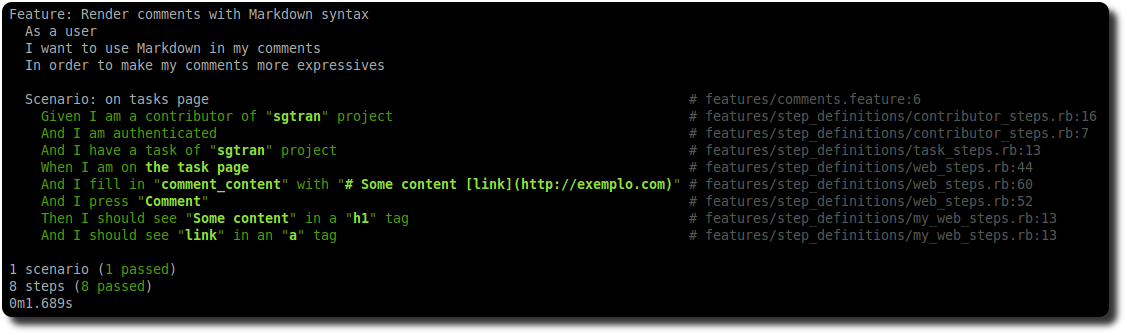
\includegraphics[scale=0.4]{images/cucumber-exec}
  \label{img:cucumber-exec}
\end{figure}


\subsubsection{Escrita em código puro}
\label{ssub:Escrita em codigo puro}

A outra maneira de escrever os testes de aceitação é com código puro. Nesta forma, todo o código dos testes (descrição e implementação) está concentrado em apenas um lugar, utilizando somente código para escrever os testes.

No Código \ref{code:bdd_spec1} pode-se ver a especificação em código puro para a funcionalidade.

\begin{mycode}{rspec}%
{Especificação em código puro}{code:bdd_spec1}
# spec/acceptance/comments_spec.rb
feature "Render comments with Markdown syntax" do
  background do
    @owner = Factory.create :contributor
    @project = Factory.create :project
    @task = Factory.create :task, :project => @project, :author => @owner
    login(@owner.email, @owner.password)
  end

  scenario "on tasks page" do
    visit project_task_path(@project, @task)
    fill_in "comment_content", :with => "# Some content [link](http://exemplo.com)"
    click_button "Comment"
    page.should have_xpath("//h1", :text => "Some content")
    page.should have_xpath("//a", :text => "link", :href => "http://exemplo.com")
  end
end
\end{mycode}

É importante ressaltar que, mesmo sem a utilização dos \textit{templates} de história e cenário, este modelo de escrita não deixa de ser BDD \cite{BDDSolis}, pois o foco da escrita dos testes continua no comportamento.

Na figura \ref{img:rspec-acceptance-exec} é apresentada a saída para a execução do teste. Neste caso, um único arquivo concentra tudo relativo ao teste.

\begin{figure}[h]
  \center
  \caption{Saída produzida pela execução dos testes utilizando escrita em código puro com RSpec + Capybara}
  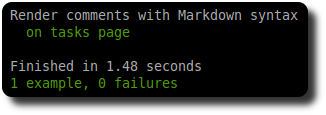
\includegraphics[scale=0.6]{images/rspec-acceptance-exec}
  \label{img:rspec-acceptance-exec}
\end{figure}


\subsubsection{Pontos em aberto sobre os modelos de escrita}
\label{ssub:pontos em aberto}

BDD vem se tornando um consenso em automação de testes. Contudo, existem uma divergência grande sobre a forma de escrita dos testes de aceitação entre escrita em código puro e escrita em texto plano, tendo alguns pontos a serem considerados.


\paragraph{Legibilidade}
\label{sssub:legibilidade}

Muitos defendem que os testes devem ser escritos em texto plano, por conta do teste ser escrito em linguagem que qualquer pessoa, mesmo sem nenhum conhecimento em programação, pode ler e validar.

Em uma situação onde se está desenvolvendo uma aplicação para um cliente, existe um mito sobre o cliente escrever as especificações, contudo está é uma abordagem utópica \cite{SteakOverCucumber, CucumberForVegetarians, ClientsWritingCucumber}. O cliente pode até ler e validar $-$ o que segundo \citeonline{YankoCapybara} nunca acontece $-$ mas mesmo assim esta não é uma abordagem muito interessante.

O cliente é especialista em problemas e os desenvolvedores em dar soluções. Se o cliente escreve a especificação, na realidade ele está escrevendo parte da solução \cite{SteakOverCucumber}. No caso da funcionalidade exemplificada anteriormente, o cliente apenas sabe que os ``comentários devem ser renderizados com markdown", ele não quer saber se para isso deve entrar em determinada página, preencher determinado campo e clicar em determinado botão. O cliente apenas sabe a funcionalidade que ele deseja, e vê-la funcionando.

Dessa forma, o cliente não tem interesse em ler a especificação como no Código \ref{code:bdd_cucumber_spec}, nem validá-la, muito menos escrevê-la. Ler somente ``Render comments with Markdown syntax" é o suficiente, mais do que isso é superficial \cite{WhyBotherWithCucumberTesting}. Os testes em texto plano se atem a detalhes de interface que são irrelevantes para os objetivos do cliente.

Uma exceção a isto ocorre em áreas que fazem uso pesado de modelagem de processo de negócio (BPM, do inglês \textit{Business Process Modeling}) \nomenclature{BPM}{Business Process Modeling} como Enterprise Information Systems, na qual descrições executáveis em texto plano podem servir como ligação entre os artefatos de BPM e o código executável \cite{IntroducingBLDD}.

Já em um contexto como o do desenvolvimento do kanban-roots, no qual não existe um cliente, onde as pessoas que escrevem e leem as especificações são desenvolvedores, a escrita em texto plano tem um valor ainda menor. O código é uma linguagem natural para desenvolvedores, ainda mais quando é escrito em conjunto com DSLs\footnote{\textit{Domain specific language} (linguagem específica de domínio) é uma linguagem de programação de expressividade limitada, focada num domínio particular.} \nomenclature{DSL}{Domain specific language} como a do Rspec \cite{SteakOverCucumber}.


\paragraph{Camada adicional}
\label{sssub:camada_adicional}

Outra crítica aos testes em texto plano é que enquanto nos testes em código puro todo o código do teste está em concentrado em apenas um lugar, nos testes em texto plano, o código do testes está espalhado em diversos arquivos e métodos, devido a camada adicional dos \textit{steps}, tonando a suíte de testes mais complexa de manter e estender \cite{SteakOverCucumber}.

Além disso, é necessário manter um segundo ambiente de testes, já que para escrever os testes de aceitação em texto plano é necessária uma ferramenta de testes específica para isso. Isso não acontece com a escrita em código puro, já que é utilizada a mesma ferramenta utilizada nos testes unitários \cite{WhyBotherWithCucumberTesting}.


\paragraph{Tempo de execução}
\label{sssub:tempo_de_execucao}

Outro questionamento é sobre a velocidade para a execução dos testes. Como o \textit{Cucumber} utiliza a \textit{Gherkin}\footnote{\url{http://github.com/cucumber/cucumber/wiki/Gherkin}}, que é uma DSL externa\footnote{Uma DSL que tem sua própria sintaxe e necessita de um \textit{parser} para processá-la \cite{DSLFowler}.}, o arquivo de \textit{features} é parseado para que os \textit{steps} sejam executados, introduzindo um tempo extra na execução dos testes.

Para um conjunto de funcionalidades, foram escritos testes utilizando os ambos modelos de escrita $-$ apresentados no Anexo \ref{cha:codigo_do_comparativo}. Cada conjunto de vinte e dois exemplos foi executado separadamente e seus tempos de execução medidos, sendo os resultados apresentados na tabela \ref{table:tempo_de_execucao}.

\begin{table}[ht]
\caption{Velocidade de execução dos testes de acordo com o método de escrita}
\label{table:tempo_de_execucao}
\centering
\begin{tabular}{p{4.5cm} p{6.5cm}}
\toprule
\textbf{Método de escrita} & \textbf{Tempo médio de execução} \\
\midrule[1pt]
texto plano & 0m11.667s \\ \midrule
código puro & 0m8.8385s \\
\bottomrule
\end{tabular}
\end{table}

Analisando estes resultados pode-se concluir que os testes em código puro executam, em média, em um tempo 25\% menor que os em texto plano.


\subsubsection{Um modelo híbrido de escrita}
\label{ssub:um_modelo_hibrido_de_escrita}

\citeonline{YankoCapybara} apresenta um modelo alternativo de escrita de testes de aceitação, sendo esta uma união entre os duas maneiras apresentadas anteriormente\footnote{Esta abordagem também é utilizada pelo \textit{framework} easyb para Java. Mais em \url{http://www.easyb.org}}. Os testes são escritos em código puro, porém utilizando \textit{steps} semelhantes aos do testes em texto plano. No código \ref{code:rspec_steps} é apresentado o exemplo anterior utilizando este novo modelo\footnote{Para a escrita deste exemplo, foi utilizada uma ferramenta criada por Yanko chamada \textit{Rspec example steps}. Mais em \url{https://github.com/railsware/rspec-example_steps}}.

\begin{mycode}{rspec}%
{Especificação mesclando código puro com texto plano}{code:rspec_steps}
feature "Render comments with Markdown syntax" do
  background do
    @owner = Factory.create :contributor
    @project = Factory.create :project
    @task = Factory.create :task, :project => @project, :author => @owner
    login(@owner.email, @owner.password)
  end

  Steps "Render on tasks page" do
    When "I am on the task page" do
      visit project_task_path(@project, @task)
    end
    And "I fill in the comment with an text with markdown syntax" do
      fill_in "comment_content", :with => "# Some content [link](http://exemplo.com)"
    end
    And "I press the Comment buttom" do
      click_button "Comment"
    end
    Then "I should see the text rendered as HTML" do
      page.should have_xpath("//h1", :text => "Some content")
      page.should have_xpath("//a", :text => "link", :href => "http://exemplo.com")
    end
  end
end
\end{mycode}

Esta abordagem busca eliminar os problemas com a camada adicional e tempo de execução que a escrita em texto plano têm. Além disso, busca também aprimorar legibilidade da documentação da escrita em código puro, pois os testes, ao serem executados, produzem uma saída como mostrado na figura \ref{img:output-novo-modelo}

\begin{figure}[h]
  \center
  \caption{Saída produzida pela execução dos testes utilizando modelo proposto por Yanko}
  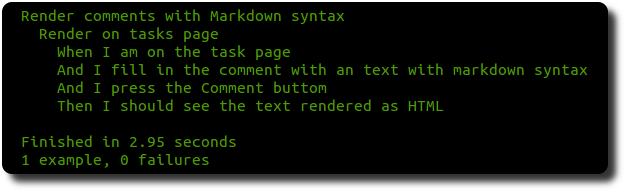
\includegraphics[scale=0.6]{images/output-novo-modelo}
  \label{img:output-novo-modelo}
\end{figure}

No entanto, esta abordagem cai no mesmo dilema da escrita em texto plano: o cliente não irá ler ou validar esta saída. Além disso, a introdução dos métodos \texttt{When/And/Then} juntamente com as \textit{strings} e blocos passados como parâmetros, piora muito a legibilidade do código de teste, prejudicando a manutenibilidade da suíte de testes. Assim, está abordagem, apesar de eliminar a camada adicional, pouco difere da escrita em texto plano, no que diz respeito às desvantagens.


\subsection{Conclusões}
\label{sub:conclusoes_bdd}

\textbf{TODO: Annabell, isso vai para as conclusões finais ou deixo aqui mesmo como uma subseção com um título diferente?}

Na opinião do autor, os testes escritos em texto plano em um primeiro momento são muito atraentes, pois, com a facilidade de leitura, a possibilidade de validação de testes executáveis pelo cliente se tornam reais. No entanto, como apresentado anteriormente, na realidade é pouquíssimo provável que o cliente irá validar estes testes. Isto é ainda mais acentuado em projetos como o kanban-roots onde não existe cliente em si, tornando totalmente irrelevante os possíveis benefícios da escrita de testes em texto plano.

Já para projetos grandes, nos quais a suíte de testes é extensa, 25\% a mais no tempo de execução dos testes é um preço alto a ser pago, pois os testes devem ser executados diversas vezes ao dia. Se o tempo necessário para executar a suíte de testes se tornar demasiadamente longo, o desenvolvedor tende a rodar os testes menos vezes, diminuindo, assim, a eficácia da aplicação do BDD. Além disso, a escrita de testes em texto plano prejudica a produtividade, pois é adicionada complexidade ao processo, devido à camada adicional, fazendo com que a produtividade seja reduzida.

Apesar dos pontos negativos, os testes em texto plano podem ter valia em situações onde o desenvolvedor tem grandes dificuldades em entender o que o cliente quer ou entender o um determinado processo realizado pelo cliente. Desta forma, o teste em texto plano pode servir como um facilitador na comunicação. Assim, sentados lado a lado, o cliente vai dizendo ao desenvolvedor qual é o fluxo, e o desenvolvedor por sua vez, vai mapeando para o teste. Como ambos conseguem ler e entender o que está sendo escrito, a discussão e entendimento do problema é facilitada.


\section{Contextualizando Integração contínua}

Nesta seção será feita uma discussão acerca das características das integrações síncrona e assíncrona, além de mostrar como a integração contínua foi feita no kanban-roots.

\subsection{Integração contínua síncrona versus assíncrona}
\label{sub:sincrona_x_assincrona}

Sempre que possível, o melhor modelo de integração a ser utilizado é o síncrono. Pode-se fazer essa afirmação baseado no que \citeonline{ArtOfAgileDevelopment} descrevem como vantagens em utilizar a integração contínua síncrona:

\begin{itemize}
  \item Se a \textit{build} falhar, não é necessário interromper uma nova tarefa iniciada para voltar e corrigir a anterior, evitando assim a mudança de contexto mental.
  \item Ajuda a manter a \textit{build} rápida, pois se está levando muito tempo para executar, a percepção é imediata e pode ser logo corrigida.
  \item A frequência de \textit{builds} quebradas é muito menor, assim o tempo de permanência da falha no sistema de controle de versão, pois o responsável pela modificação que introduziu a falha pode não estar apto para corrigir-la imediatamente.
\end{itemize}

\citeonline{ImproveitCI} corrobora dizendo que a integração contínua assíncrona permite o trabalho de desenvolvedores distribuídos geograficamente, porém é um pouco mais arriscada e menos eficiente que a integração síncrona. O risco aumenta porque o repositório pode ficar inconsistente durante alguns períodos de tempo $-$ sempre que um erro ocorre e o responsável por ele ainda não fez o \textit{commit} das correções. Na integração assíncrona, a eficiência diminui porque leva mais tempo para o desenvolvedor descobrir que cometeu um erro. É comum o desenvolvedor receber a notificação de um erro depois de já ter iniciado uma nova atividade. Ao ser notificado, deve parar a nova tarefa, relembrar o que havia feito na tarefa anteriormente e corrigir o erro. O processo síncrono é mais eficiente no uso do \textit{feedback} exatamente porque impede o desenvolvedor de desviar sua atenção para qualquer outra atividade, enquanto a integração não tiver sido concluída com sucesso.


\subsection{Integração contínua no kanban-roots}
\label{sub:integracao_continua_no_kanban}

Com base no tópico anterior e por ser um projeto \textit{open source}, no kanban-roots foi utilizado o método assíncrono de integração contínua, através do Travis\footnote{Mais informações podem ser encontradas em \url{http://travis-ci.org}}, que foi escolhido por ser um serviço hospedado e gratuito de integração contínua para a comunidade \textit{open source}, o que facilitou bastante pela não necessidade de manutenção de uma estrutura local de integração contínua. Na Figura \ref{img:travis-success} é apresentada a tela do Travis quando a \textit{build} é executada com sucesso e na Figura \ref{img:travis-fail} quando a \textit{build} falha.

\begin{figure}[h]
  \center
  \caption{Tela do Travis quando a \textit{build} é executada com sucesso}
  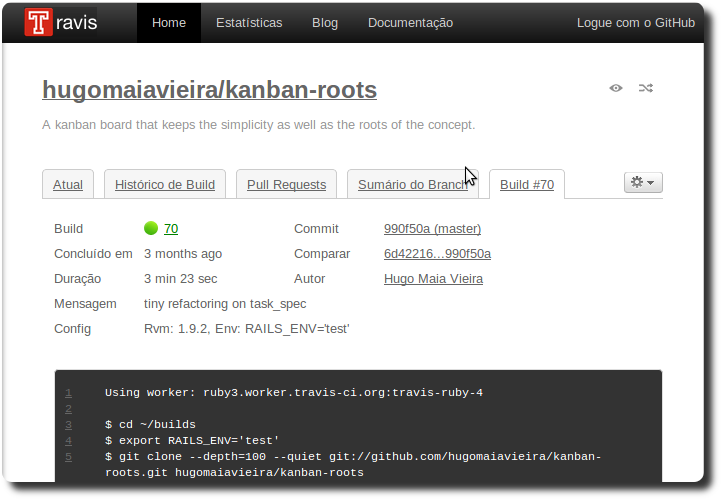
\includegraphics[scale=0.55]{images/travis-success}
  \label{img:travis-success}
\end{figure}

Na Seção \ref{sec:contextualizando_tdd} sobre testes de integração, foi apresentado o Código \ref{code:integration_spec3} com os testes de integração para o \textit{highlighting} de código. Para que a integração contínua pudesse continuar sendo executada no Travis, o teste que verifica a integração do kaban-roots com o Pygments local foi comentado, uma vez que não é possível fazer instalações de dependências de sistema no Travis. Neste caso, o ideal seria ter um servidor próprio para rodar a integração contínua, pois esta tem que simular um ambiente de produção da forma mais perfeita possível, utilizando o Jenkins\footnote{Mais informações em \url{http://jenkins-ci.org/}} por exemplo.

\begin{figure}[h]
  \center
  \caption{Tela do Travis quando a \textit{build} falha}
  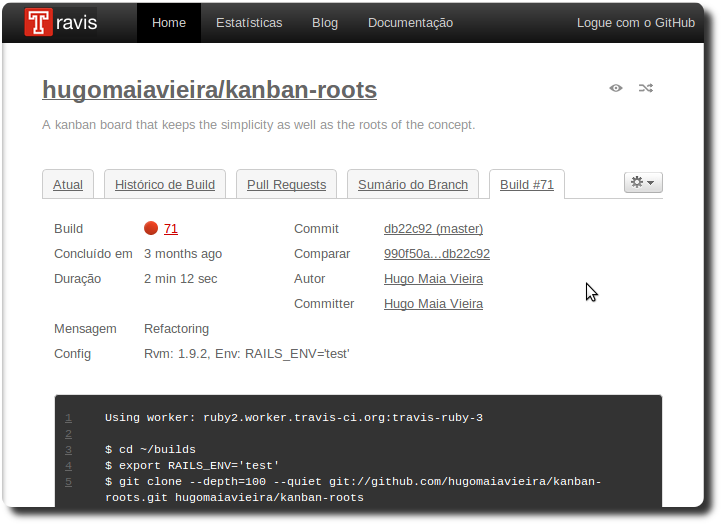
\includegraphics[scale=0.55]{images/travis-fail}
  \label{img:travis-fail}
\end{figure}

A integração contínua se mostrou importante em algumas ocasiões durante o desenvolvimento do kanban-roots, a exemplo:

\begin{itemize}
  \item Alguns arquivos não foram incluídos no \textit{commit}, fazendo com que localmente tudo funcionasse perfeitamente, mas o repositório estava quebrado.
  \item Em ambiente de desenvolvimento é utilizado o SQLite\footnote{\url{http://www.sqlite.org}} e em ambiente de produção, é utilizado o MySQL\footnote{\url{http://www.mysql.com}}. Assim, foi feita uma \textit{query} que apenas funcionava no SQLite, mas não no MySQL. Ou seja, em desenvolvimento estava perfeito, mas em produção, não.
\end{itemize}

Com o \textit{feedback} rápido da integração contínua, todas as falhas foram corrigidas muito rapidamente, sem que problemas maiores ocorressem e outras modificações na base de código fossem feitas sobre as modificações problemáticas, o que faria com que a correção dos problemas fosse mais complexa e levasse mais tempo.


\section{Contextualizando dublês de teste}

Nesta seção será feita a contextualização dos dublês de teste \textit{stub} e \textit{mock}, com exemplos de utilização no kanban-roots. Além disso, será feita uma discussão sobre a dicotomia entre o TDD clássico e o mockista.

\subsection{Contextualizando o \textit{stub}}
\label{sub:contextualizando_o_stub}

Um exemplo da utilização simples e eficiente do \textit{stub} foi mostrado no teste de integração apresentado na Seção \ref{sec:contextualizando_tdd}. Naquele exemplo, foi feito um \textit{stub} do método \texttt{can\_pygmentize?} que faz uma consulta ao sistema operacional para verificar se uma determinada dependência de sistema está instalada. Desta forma, o teste ficou isolado, não importando se a máquina em que o teste for executado tem ou não a dependência instalada, sendo assim possível simular as duas situações $-$ logicamente, uma maquina não pode, ao mesmo tempo, ter e não ter uma dependência instalada.

Um outro exemplo é mostrado no Código \ref{code:stub_spec}, onde está sendo testada uma ação da classe \textit{Project}. Contudo, para que esta ação seja realizada, é necessário um conjunto de objetos da classe \textit{Task}. Assim, com o objetivo de criar um teste isolado e concentrado na classe \textit{Project}, é utilizado o método \texttt{stub\_model} que cria um \textit{stub} da classe \textit{Task} que irá reponder apenas aos atributos definidos no \textit{hash} passado como segundo parâmetro. No caso, a ação em questão é contar a soma dos pontos das tarefas alocadas em uma determinada posição do quadro (kanban). Esta ação é exercida através do método \texttt{count\_points}, cuja implementação é apresentada no Código \ref{code:stub}. Na Figura \ref{img:count-points} é apresentada uma utilização do método \texttt{count\_points} no somatório de pontos das tarefas na posição \textit{To Do} do kanban.

\begin{mycode}{rspec}%
{Exemplo do \textit{stub} da classe \textit{Task}}{code:stub_spec}
# spec/models/project_spec.rb
describe Project do
  it "returns the tasks points sum for a given position of the board" do
    tasks = [stub_model(Task, :points => 1, :position => Board::POSITIONS["doing"]),
             stub_model(Task, :points => 2, :position => Board::POSITIONS["doing"]),
             stub_model(Task, :points => 8, :position => Board::POSITIONS["todo"]),
             stub_model(Task, :points => nil, :position => Board::POSITIONS["todo"]),
             stub_model(Task, :points => 3, :position => Board::POSITIONS["doing"]),
             stub_model(Task, :points => 5, :position => Board::POSITIONS["todo"])]
    project = Project.new
    project.tasks.<<(*tasks)

    project.count_points(Board::POSITIONS["todo"]).should == 13
    project.count_points(Board::POSITIONS["doing"]).should == 6
    project.count_points(Board::POSITIONS["done"]).should == 0
  end
end
\end{mycode}

\begin{mycode}{ruby}%
{Implementação do método \texttt{Project\#count\_points}}{code:stub}
# app/models/project.rb
class Project
  def count_points position
    points = 0
    self.tasks_by_position(position).each do |task|
      points += task.points if task.points
    end
    points
  end
end
\end{mycode}

\begin{figure}[h]
  \center
  \caption{Utilização do método \texttt{count\_points} no somatório de pontos das tarefas de uma posição}
  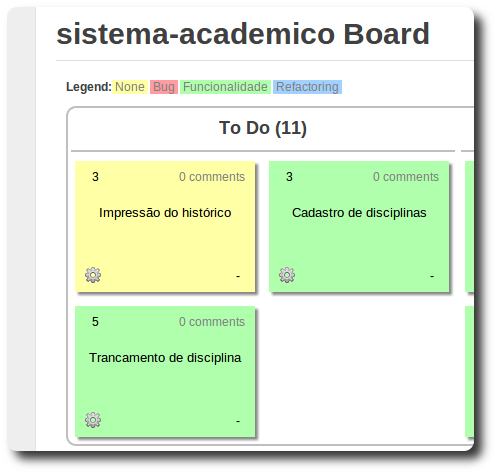
\includegraphics[scale=0.5]{images/count-points}
  \label{img:count-points}
\end{figure}

Contudo, a utilização desta técnica deve ser feita com cautela. Quando se utiliza \textit{stubs} em demasia, cria-se um acoplamento muito grande entre teste e implementação. Por exemplo, se na implementação do método \texttt{count\_points} for preciso fazer uso de mais algum atributo de \textit{Task} (em uma refatoração, por exemplo), o \textit{stub} também deverá possuir esse atributo, fazendo com que o teste tenha que ser alterado. Isso vai contra uma das premissas da refatoração de que se o comportamento do método não é modificado, seu teste deve permanecer o mesmo e continuar passando após ser feita a alteração na implementação.

É importante notar a diferença entre os \textit{stubs} e as estratégias de \textit{fixture replacement}\footnote{\textit{Fixture replacement} é uma técnica que tem como objetivo separar a inicialização do teste de sua codificação em si, dando a possibilidade de se criar objetos com estados pré-definidos que possam ser reutilizados em mais de um teste.} baseadas em instâncias. Nestas estratégias, o \textit{fixture} é um objeto real da classe. Assim, um objeto criado via \textit{fixture replacement} de instância, fica sujeito a detalhes de sua implementação da classe real. Dessa forma, o {fixture} não cria o isolamento que um \textit{stub} em seu lugar criaria, pois o stub simplesmente simula uma instância e, portanto, não fica sujeito comportamentos inesperados.


\subsection{Contextualizando o \textit{mock}}
\label{sub:contextualizando_o_mock}

De modo semelhante ao Código \ref{code:todo} apresentado na Seção \ref{sub:a_ubiquidade_do_tdd}, o Código \ref{code:mock} apresenta a implementação de um método de \textit{controller} que é chamado via AJAX (\textit{Asynchronous Javascript and XML})\nomenclature{AJAX}{Asynchronous Javascript and XML} e implementa a atualização dos responsáveis por uma tarefa diretamente do kanban do projeto, como apresentado na Figura \ref{img:edit-contributors}. Além atualizar os responsáveis pela tarefa tarefa na base de dados, este método captura, trata e envia informações para que a interface do kanban seja atualizada. Este é outro caso onde um experimento foi para produção, sem testes e com um código ruim. Desta forma, neste caso não foi utilizado TDD para criar os testes, sendo estes escritos após a implementação.

\begin{mycode}{ruby}%
{Código do método que atualiza os responsáveis por uma tarefa assincronamente}{code:mock}
# app/controllers/boards_controller.rb
class BoardsController < InheritedResources::Base
  # TODO: Make test and refactor
  def update_assignees
    task = Task.find(params[:task_id])
    params[:assignees].delete "-"
    params[:assignees] = nil if params[:assignees].empty?
    task.update_attribute(:contributor_ids, params[:assignees])

    if params[:assignees].nil?
      assignees_sentence = "-"
    else
      assignees_sentence = task.contributors.collect(&:username).to_sentence
    end

    if assignees_sentence.length > 25
      long_sentence = true
      assignees_long_sentence = assignees_sentence
      assignees_sentence = assignees_sentence.truncate(25)
    end

    data = { :assignees_sentence => assignees_sentence,
             :long_sentence => long_sentence,
             :assignees_long_sentence => assignees_long_sentence }
    render :text => data.to_json
  end
end
\end{mycode}

\begin{figure}[h]
  \center
  \caption{Atualização dos responsáveis pela tarefa diretamente no kanban do projeto}
  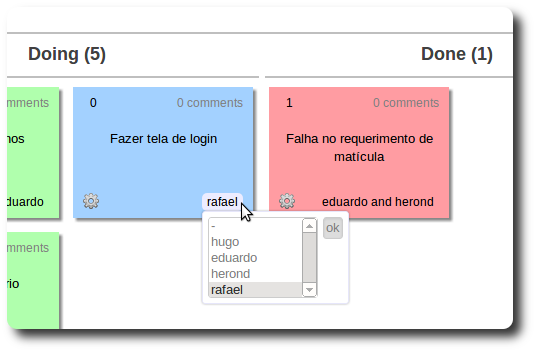
\includegraphics[scale=0.55]{images/edit-contributors}
  \label{img:edit-contributors}
\end{figure}

O teste para o método \texttt{update\_assignees}, com a utilização de \textit{mock}, é apresentado no Código \ref{code:mock_spec_mockista}. Como o teste quer validar a funcionalidade para mais de um responsável (\textit{assignees}), são criados dois objetos mockados da classe \textit{Contributor}, além de também ser necessário cria um objeto mockado da classe \textit{Task}. Com esses 3 objetos mockados, está feito a \textit{setup} para o teste.

Em seguida verificadas as chamadas à métodos sobre os objetos mockados. Isto é feito através do método \texttt{should\_receive} que recebe como parâmetro o método a ser chamado. Em seguida, pode ser aninhado o método \texttt{with} que recebe os parâmetros que devem ser passados para o método chamado no \texttt{should\_receive}. Para finalizar a cadeia, pode ser ainda aninhado o método \texttt{and\_return} que indica o retorno do método chamado no \texttt{should\_receive}.

Por fim, através de um \texttt{get}, é feita a chamada ao método do \textit{controller} testado (\texttt{update\_assignees}), e é verificado se a resposta obtida está de acordo com as expectativas.

\begin{mycode}{rspec}%
{Teste utilizando \textit{mock} para o método \texttt{update\_assignees}}{code:mock_spec_mockista}
# spec/controllers/boards_controller_spec.rb
describe BoardsController do
  context "should update task assignees" do
    it "with more than one assignee" do
      task = mock_model(Task)
      hugo = mock_model(Contributor, :id => "5", :username => "hugomaiavieira")
      rodrigo = mock_model(Contributor, :id => "9", :username => "rodrigomanhaes")

      Task.should_receive(:find).with("1").and_return(task)
      task.should_receive(:update_attribute).
        with(:contributor_ids, ["5", "9"]).and_return(true)
      task.should_receive(:contributors).and_return([hugo, rodrigo])

      get :update_assignees, :task_id => "1", :assignees => ["5", "9"]

      response.body.should ==
        { :assignees_sentence => "hugomaiavieira and rod...",
          :long_sentence => true,
          :assignees_long_sentence => "hugomaiavieira and rodrigomanhaes" }.to_json
    end
  end
end
\end{mycode}

O grande problema do mock está nas verificações de chamada à métodos dos objetos mockados. Pose-se perceber que está se verificando a ordem em que os métodos são chamados, bem como os parâmetros passados. Desta forma, na realidade, está se testando \textbf{como} a funcionalidade está sendo implementada e não \textbf{o que} ela faz \cite{UnitForAReason}. Com isso, o acoplamento entre o teste e a implementação torna-se extremamente grande, ainda maior do que com a utilização de \textit{stubs}. Qualquer refatoração mínima feita na implementação, mesmo que não interfira em seu comportamento, pode fazer com que os testes quebrem.

Para fazer uma comparação, no Código \ref{code:mock_spec_tradicional} é apresentado um outro teste para o mesmo exemplo, porém, utilizando objetos reais criados através de \textit{fixture replacement}. Note que desta vez foi preciso criar um objeto \textit{Project} para ligar ao objeto \textit{task}, pois quando são utilizados objetos reais, todas as validações são executadas e, neste caso, uma tarefa obrigatoriamente deve estar ligada a um projeto.

\begin{mycode}{rspec}%
{Teste utilizando \textit{fixture replacement} para o método \texttt{update\_assignees}}{code:mock_spec_tradicional}
# spec/controllers/boards_controller_spec.rb
describe BoardsController do
  context "should update task assignees" do
    it "with more than one assignee" do
      project = Factory.create :project
      task = Factory.create :task, :project => project
      hugo = Factory.create :contributor, :username => "hugomaiavieira"
      rodrigo = Factory.create :contributor, :username => "rodrigomanhaes"

      get :update_assignees, :task_id => task.id, :assignees => [hugo.id, rodrigo.id]

      response.body.should ==
        { :assignees_sentence => "hugomaiavieira and rod...",
          :long_sentence => true,
          :assignees_long_sentence => "hugomaiavieira and rodrigomanhaes" }.to_json
    end
  end
end
\end{mycode}

Percebe-se que o teste sem o uso do \textit{mock} fica mais simples e menos acoplado à implementação. Contudo, o teste usando \textit{mock} ganhou um isolamento maior por não ficar sujeito a detalhes da implementação das classes, irrelevantes para o teste. Além disso, os testes utilizando mock rodaram com uma velocidade 58\% maior do que o teste sem \textit{mock}. Isso acontece porque os testes sem \textit{mock} (utilizando \textit{fixture replacement}) fazem acesso ao disco para gravar as informações dos objetos reais no banco de dados de teste.


\subsection{A dicotomia entre o TDD clássico e o mockista}
\label{sub:tdd_classico_e_mockista}

\citeonline{MocksArentStubs} generaliza os dublês de teste como \textit{mocks} e define duas faces da sua utilização com TDD, onde o divisor é \textbf{quando} utilizar um dublê:

\begin{itemize}
  \item O estilo \textbf{TDD clássico} é o qual se utiliza objetos reais sempre que possível e dublês quando é complicado utilizar o real.

  \item O estilo \textbf{TDD mockista} (\textit{mockist}, em inglês) é o qual se utiliza dublês sempre.
\end{itemize}

Como visto anteriormente, a utilização de dublês de teste, em alguns casos, é claramente benéfica para o projeto. Porém, seu uso excessivo pode causar um problema de acoplamento entre o teste e a implementação.

\citeonline{ArtOfAgileDevelopment} afirma o \textit{mock} é uma técnica útil, e as vezes é a melhor maneira de testar o código. No entanto, ele diz que antes de assumir que o \textit{mock} é apropriado para a situação, deve-se olhar novamente para o design do código, pois pode ser uma oportunidade de aprimoramento.

Uma outra questão a ser levada em consideração é que quando não se utiliza dublês, está se testando a integração entre as classes, e isso pode ter um efeito colateral positivo, capturando erros que muitas vezes passam despercebidos ao se utilizar \textit{dublês}. Contudo, quando não se utiliza dublês, para testar uma unidade pode ser necessário desenvolver outras unidades colaboradoras, cada qual com seus correspondentes testes de unidade, assim tirando o foco da tarefa corrente.

Dessa forma, assim como \citeonline{MocksArentStubs} conclui, não existe razão para adotar um estilo TDD mockista, sendo o TDD clássico a melhor opção, utilizando os dublês de teste de forma controlada.